% このファイルは自動生成されました
% 親ファイル(tex_soturonhappyoルート)から \input して使用することを想定しています

% フレーム1: フィボナッチ法（補足1）
\begin{frame}
  \frametitle{フィボナッチ法による最適探索}
  \begin{columns}
    \begin{column}{0.45\textwidth}
      \small
      \textbf{補足：} Kiefer氏は観測回数が固定された場合、フィボナッチ数を用いた探索法を提示しました。
      
      \vspace{0.5em}
      \begin{itemize}
        \item 観測回数が\textbf{事前に決定}されている
        \item フィボナッチ数により最悪ケースを最適化
        \item 関数値が小さい側に拡大
        \item 赤点：新規評価点
      \end{itemize}
      
      \vspace{0.5em}
      \textbf{目的関数:} $f(x) = (x-2)^2 + 0.5\sin(3x)$
    \end{column}
    \begin{column}{0.55\textwidth}
      \centering
      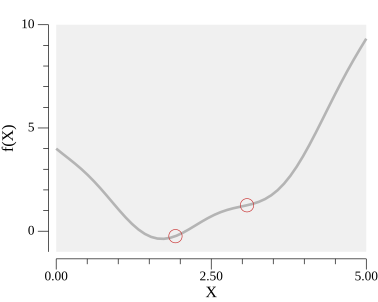
\includegraphics[width=\textwidth]{material/kiefer/output/fibonacci_fixed_obs.png}
    \end{column}
  \end{columns}
\end{frame}

% フレーム2: 黄金比を用いた方法（補足2）
\begin{frame}
  \frametitle{黄金比を用いたアルゴリズム}
  \begin{columns}
    \begin{column}{0.45\textwidth}
      \small
      \textbf{補足：} これとは別に、黄金比を用いて常に同じアルゴリズムで区間を縮小する手順が提示されました。
      
      \vspace{0.5em}
      \begin{itemize}
        \item 黄金比 $\phi = \frac{\sqrt{5}-1}{2} \approx 0.618$
        \item \textbf{同じアルゴリズム}を繰り返す
        \item 観測回数は事前に決めない
        \item 関数が単峰性を保つ限り有効
      \end{itemize}
      
      \vspace{0.5em}
      これが一般に\textbf{黄金分割法}と呼ばれます。
    \end{column}
    \begin{column}{0.55\textwidth}
      \centering
      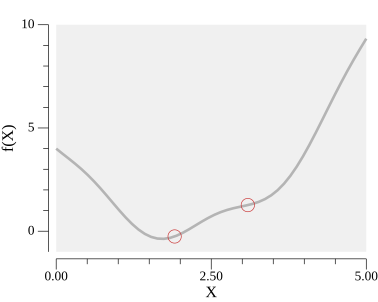
\includegraphics[width=\textwidth]{material/kiefer/output/golden_ratio_method.png}
    \end{column}
  \end{columns}
\end{frame}

% フレーム3: 黄金分割法の実用性（補足3）
\begin{frame}
  \frametitle{黄金分割法の実用性}
  \begin{columns}
    \begin{column}{0.45\textwidth}
      \small
      \textbf{補足：} 黄金分割法は厳密には最適な手順ではありませんが、観測回数を事前に決めない場合に特に有用です。
      
      \vspace{0.5em}
      \begin{itemize}
        \item 各段階で区間は最悪でも $0.618$ 倍に縮小する
        \item 実装が簡単で安定している
        \item 収束性が良好
        \item 観測回数を任意に変更可能
      \end{itemize}
      
      \vspace{0.5em}
      \textbf{利点:} 実用性と安定性のバランスが優れている
    \end{column}
    \begin{column}{0.55\textwidth}
      \centering
      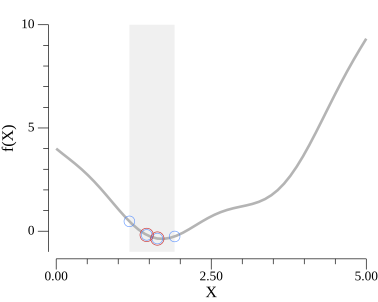
\includegraphics[width=\textwidth]{material/kiefer/output/golden_section_no_fixed_obs.png}
    \end{column}
  \end{columns}
\end{frame}

